
%%%%%%%%%%%%%%%%%%%%%%%%%%%%%%%%%%%%%%%%%%%%%%%%%%%%%%%%%%%%%%%%%%%%%%%%%%%%%%
%  ************************** AVISO IMPORTANTE **************************    %
%                                                                            %
% Éste es un documento de ayuda para los autores que deseen enviar           %
% trabajos para su consideración en el Boletín de la Asociación Argentina    %
% de Astronomía.                                                             %
%                                                                            %
% Los comentarios en este archivo contienen instrucciones sobre el formato   %
% obligatorio del mismo, que complementan los instructivos web y PDF.        %
% Por favor léalos.                                                          %
%                                                                            %
%  -No borre los comentarios en este archivo.                                %
%  -No puede usarse \newcommand o definiciones personalizadas.               %
%  -SiGMa no acepta artículos con errores de compilación. Antes de enviarlo  %
%   asegúrese que los cuatro pasos de compilación (pdflatex/bibtex/pdflatex/ %
%   pdflatex) no arrojan errores en su terminal. Esta es la causa más        %
%   frecuente de errores de envío. Los mensajes de "warning" en cambio son   %
%   en principio ignorados por SiGMa.                                        %
%                                                                            %
%%%%%%%%%%%%%%%%%%%%%%%%%%%%%%%%%%%%%%%%%%%%%%%%%%%%%%%%%%%%%%%%%%%%%%%%%%%%%%

%%%%%%%%%%%%%%%%%%%%%%%%%%%%%%%%%%%%%%%%%%%%%%%%%%%%%%%%%%%%%%%%%%%%%%%%%%%%%%
%  ************************** IMPORTANT NOTE ******************************  %
%                                                                            %
%  This is a help file for authors who are preparing manuscripts to be       %
%  considered for publication in the Boletín de la Asociación Argentina      %
%  de Astronomía.                                                            %
%                                                                            %
%  The comments in this file give instructions about the manuscripts'        %
%  mandatory format, complementing the instructions distributed in the BAAA  %
%  web and in PDF. Please read them carefully                                %
%                                                                            %
%  -Do not delete the comments in this file.                                 %
%  -Using \newcommand or custom definitions is not allowed.                  %
%  -SiGMa does not accept articles with compilation errors. Before submission%
%   make sure the four compilation steps (pdflatex/bibtex/pdflatex/pdflatex) %
%   do not produce errors in your terminal. This is the most frequent cause  %
%   of submission failure. "Warning" messsages are in principle bypassed     %
%   by SiGMa.                                                                %
%                                                                            % 
%%%%%%%%%%%%%%%%%%%%%%%%%%%%%%%%%%%%%%%%%%%%%%%%%%%%%%%%%%%%%%%%%%%%%%%%%%%%%%

\documentclass[baaa]{baaa}
 
%%%%%%%%%%%%%%%%%%%%%%%%%%%%%%%%%%%%%%%%%%%%%%%%%%%%%%%%%%%%%%%%%%%%%%%%%%%%%%
%  ******************** Paquetes Latex / Latex Packages *******************  %
%                                                                            %
%  -Por favor NO MODIFIQUE estos comandos.                                   %
%  -Si su editor de texto no codifica en UTF8, modifique el paquete          %
%  'inputenc'.                                                               %
%                                                                            %
%  -Please DO NOT CHANGE these commands.                                     %
%  -If your text editor does not encodes in UTF8, please change the          %
%  'inputec' package                                                         %
%%%%%%%%%%%%%%%%%%%%%%%%%%%%%%%%%%%%%%%%%%%%%%%%%%%%%%%%%%%%%%%%%%%%%%%%%%%%%%
 
\usepackage[pdftex]{hyperref}
\usepackage{subfigure}
\usepackage{natbib}
\usepackage{helvet,soul}
\usepackage[font=small]{caption}
\usepackage[portuguese]{babel}
\usepackage{physics,elements}
\usepackage{siunitx,lipsum}
\usepackage[T1]{fontenc}


\contriblanguage{0}



\contribtype{8}



\thematicarea{99}


\title{Análise de interface SiO2/Si\\através de espectro de XPS}



\titlerunning{Análise de Superfícies}



\author{
Gonçalo G. Baptista\inst{1}
}

\authorrunning{Gonçalo Baptista}


\contact{g.baptista@campus.fct.unl.pt}



\institute{
NOVA School of Science and Technology, NOVA SST, Portugal
}



\resumen{Neste trabalho irá proceder-se à análise de um espetro de XPS adquirido a partir da irradiação de uma interface SiO$_2$/Si com orientação (111) usando um feixe de fotões com energia de $130\ \si{\electronvolt}$, sendo neste caso estudadas as \textit{binding energies} das orbitais 2p. Ao espetro obtido será realizado um fit que englobe as diferentes contribuições dos diversos estados de oxidação do Si e posteriormente a determinação da estequiometria e espessura de cada uma das camadas presentes.}

\abstract{In this project, we will analyse a XPS spectrum aquired during the irradiation of a SiO$_2$/Si (111) interface using an $130\ \si{\electronvolt}$ X-Ray photon beam. This spectrum is related to the 2p orbitals' binding energies of multiple Si oxydated states which will be taken into account whilst performing fitting routines to the data that will then be used in the determination of the sample's stoichiometry and thickness.}



\keywords{ Espetroscopia XPS --- SiO2 --- Estados de Oxidação}


\begin{document}

\maketitle

\section{Introdução}\label{S_intro}

Para a realização deste trabalho foi fornecido um espetro experimental de espectroscopia do tipo XPS\footnote{X-ray Photoelectron Spectroscopy}, em que se irradiou uma amostra de Si (111) com fotões de $130\ \si{\electronvolt}$ e se analisaram \textit{core levels} do Si. Este espectro foi obtido através de um varrimento de energias com passos de $20\ \si{\milli\electronvolt}$, permitindo analisar \textit{binding energies} dos $96$ aos $98\ \si{\electronvolt}$. Tal \textit{range} corresponde às \textit{binding energies} das orbitais 2p 3/2 e 2p 1/2 de diversos estados de oxidação do Si. Tais orbitais foram escolhidas devido ao facto de no SiO$_2$ ocorrerem 2 ligações duplas e sendo a configuração eletrónica do Si \elconf{Si}, os 4 eletrões menos ligados, ou seja, das orbitais 3p e 3s irão participar nas duas ligações duplas. Sendo assim, a orbital 2p será a orbital menos ligada do sistema no seu maior estado de oxidação.


\section{Tratamento de Dados}
Para todo o tratamento de dados recorreu-se à utilização de um \textit{software} próprio para análise de espetros de XPS, o \textit{CasaXPS}. Tal deve-se ao facto de possuir um inúmero conjunto de ferramentas de remoção de fundo e rotinas de \textit{fitting} que serão uma mais valia na seguinte análise.


\subsection{Remoção de Fundo}

Para se proceder a um tratamento correto dos dados e à procedente interpretação de resultados, será de elevada importância remover o fundo presente no espetro. Tendo em conta o espetro obtido e a aparente forma do fundo, escolheu-se usar um \textit{background} dos estilo \textit{Tougaard}. Selecionou-se um \textit{range} de energias de modo a englobar os picos da 2p obtidos mas excluindo um pequeno pico presente em valores de \textit{binding energy} mais altos devido a um plasmão. na Fig. \ref{fig:bgrm} pode encontrar-se o processo de remoção de fundo.


\begin{figure}[t!]
    \centering
    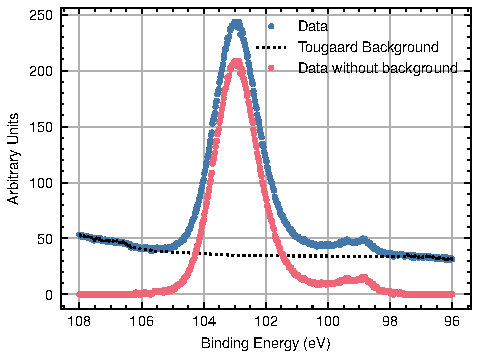
\includegraphics[width=\columnwidth]{Figuras/data_init.pdf}
    \caption{Dados com e sem Background removido}
    \label{fig:bgrm}
  \end{figure}

\subsection{Desconvolução de picos}

Observando-se a Fig. \ref{fig:bgrm} rapidamente se identifica 1 pico bem definido\footnote{São, na realidade, vários picos convoluídos}. No entanto também se observa a presença de uma estrutura de forma irregular entre os 98 e os $100\ \si{\electronvolt}$. É necessário compreender, distinguir e quantificar as contribuições que os diferentes estados de oxidação do Si têm nestas estruturas. Considerou-se, inicialmente a existência de Si em 5 estados diferentes: Si, Si$^{+1}$, Si$^{+2}$, Si$^{+3}$, Si$^{+4}$\footnote{Corresponde a SiO$_2$}. Os valores de \textit{binding energy} para os diferentes estados de oxidação foram inicialmente adaptados de \cite{Himpsel}, mas através de rotinas de \textit{fitting}, encontraram-se os valores ótimos para este caso. Tendo em conta que as orbitais em estudo são do tipo p (l=1) e que os eletrões possuem momento angular intrínseco (s=1/2), irão  existir \textbf{sempre} 2 tipos de acoplamento de momento angular possíveis $\qty(1\pm 1/2)$: 1/2 e 3/2. É possível também saber a razão entre a área dos picos para este acoplamento, devido ao número de estados de ocupação para cada um:


\begin{itemize}
  \item p 1/2$\longrightarrow 2\cdot 1/2 +1 = 2$ eletrões
  \item p 3/2$\longrightarrow 2\cdot 3/2 +1 = 4$ eletrões
\end{itemize}


Logo, será de esperar que a intensidade dos picos referentes a 2p 3/2 seja o dobro dos referentes a 2p 1/2. Também é conhecido, para o Si que, por norma existe uma diferença de $0.6\ \si{\electronvolt}$ entre os acoplamentos. Estes 2 factos referidos anteriormente foram usados como \textit{constraints} aquando a realização dos \textit{fits}.

\begin{figure}[t!]
  \centering
  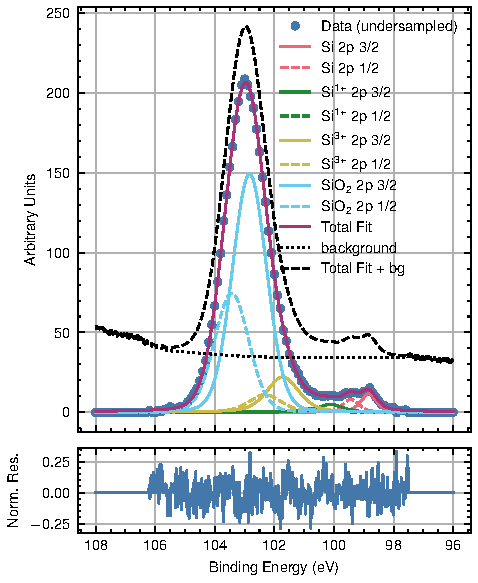
\includegraphics[width=\columnwidth]{Figuras/fits.pdf}
  \caption{Componentes e Fit total}
  \label{fig:tot}
\end{figure}


Observou-se que, para além de quase todo o Si na interface se encontrar completamente oxidado (Si$^{+4}$), ainda se encontra a presença de Si, Si$^{+1}$ e Si$^{+3}$, notando-se a ausência de Si$^{+2}$. Tendo em conta que as linhas possuem diferentes proporções de componentes Gaussianas e Lorentzianas, definiu-se que, a componente Gaussiana aumenta com a energia e fixou-se que os acoplamentos possuiam o mesmo tipo de linha e a mesma FWHM.

\begin{table}[h!]
  \centering
  \caption{Parâmetros do fit para as orbitais 2p 3/2 e comparação com valores de referência\cite{Nist}. É possível calcular-se os parâmetros das orbitais 2p 1/2 somando $0.6\ \si{\electronvolt}$ às Energias/centroides e dividindo as intensidades por um fator de 2. Os restantes parâmetros são os mesmos. O tipo de linha usado representa uma \textit{pseudo-voigt}, definida como a soma de uma Gaussiana com uma Lorentziana, neste caso com os mesmos parâmetros de média e desvio padrão, sendo o parâmetro usado o peso da parte Lorentziana. Ex:$SGL\qty(x)=\qty(1-0.01\cdot x) G + 0.01\cdot x$ L}
  \begin{tabular}{lccccc}
    \hline\hline\noalign{\smallskip}
    State & Energy &En. Diff.& FWHM& Intensity&Line\\
    & $\qty(\si{\electronvolt})$&$\qty(\si{\electronvolt})$& $\qty(\si{\electronvolt})$& (Arb. u.)&Type\\
    \hline\noalign{\smallskip}
    Si &98.85&& 0.657 &10.087&SGL(50)\\
    Si$^{1+}$&99.99&& 1.299 & 8.0485&SGL(40)\\
    Si$^{3+}$&101.77&&1.329&37.911&SGL(30)\\
    SiO$_2$ & 102.84&&1.341&221.6&SGL(10)\\
    \hline
    \end{tabular}
    \label{table:params}
\end{table}


Os resultados obtidos (Tab. \ref{table:params} e Fig. \ref{fig:tot}) fazem sentido visto que, a remoção de eletrões no processo de oxidação leva a uma menor energia de repulsão entre os restantes (sendo esta convencionalmente positiva), levando a um aumento da \textit{binding energy} para estados mais oxidados. Também se observa que a FWHM, tal como a componente Gaussiana, aumentam com o estado de oxidação. Tal pode dever-se ao aumento da complexidade do sistema, devido à ligação entre os átomos. Também é de referir que os valores divergem ligeiramente de \cite{Himpsel} devido a diferentes contribuições de Estado Sólido.



\section{Quantificação}

\subsection{Cálculo da estequiometria}

Procedeu-se ao cálculo da estequiometria da interface com base numa simples aproximação mencionada em \cite{Himpsel}. Serão calculados os pesos de cada uma das intensidades sendo necessário primeiro proceder à sua normalização com base nas secções eficazes de ionização. Resumidamente:

\begin{gather}
  x_i= \qty(\frac{I_i}{\sigma_i})\cdot\qty(\sum_i^n \frac{I_i}{\sigma_i})^{-1}
  \label{eq:quant}
\end{gather}

Os valores de $\sigma_i$ representam a secção eficaz de fotoionização da orbital 2p para o estado de oxidação $i$ normalizada em relação à para o Si neutro e, para uma energia de feixe de $130\ \si{\electronvolt}$ foram consultados em \textit{TABLE II} de \cite{Himpsel}. Tendo em conta a Eq. \ref{eq:quant}, é possível calcular-se agora a estequiometria do sistema. Esta será calculada (Tab. \ref{table:esteq})para o sistema no seu total, $x_i$ tot., (Si totalmente oxidado, os diferentes estados de oxidação e Si neutro) e para o sistema em estado de oxidação, $x_i$ oxi., (totalmente oxidado e oxidações parciais). Tal deve-se ao facto de se considerarem 2 layers na amostra (uma superficial, contendo os estados de oxidação, e outra contendo Si puro). Mais uma vez esta análise apenas será realizada para os acoplamentos 2p 3/2 devido ao facto de o resultado ser o mesmo caso fossem considerados tambem os 2p 1/2, devido à \textit{constraint} imposta aquando o processo de \textit{fitting}, onde se forçaram estes a possuir metade da intensidade dos anteriores.




\begin{table}[h!]
  \centering
  \caption{Quantificação da presença de diferentes estados de oxidação na amostra}
  \begin{tabular}{lccccc}
    \hline\hline\noalign{\smallskip}
    State & $I_i$ &$\sigma_i$& $I_i/\sigma$& $x_i$ tot.&$x_i$ oxi.\\
    \hline\noalign{\smallskip}
    Si &10.087&1& 10.087&7.15\%&---\\
    Si$^{1+}$&8.045&1.0& 8.045 &5.70\% &6.14\%\\
    Si$^{3+}$&37.911&1.7&22.300&15.80\%&17.02\%\\
    SiO$_2$ &221.6&2.2&100.7&71.35\%&76.84\%\\
    \hline
    \end{tabular}
    \label{table:esteq}
\end{table}


Conclui-se, tal como esperado, que a grande maioria da amostra se encontra totalmente oxidada e mais de $90\%$ em pelo menos um estado de oxidação.

\subsection{Determinação da espessura da amostra}

Em \cite{Himpsel} é referênciada a seguinte expressão que permite relacionar razão entre as intensidades, $I$, dos estados e máxima oxidação (SiO$_2$) e oxidação nula (Si) com a \textit{escape depth}, $l$, de tanto o Si como o SiO$_2$, as secções eficazes de fotoionização, $\sigma$, e a espessura da amostra, $d$:

\begin{gather}
  \frac{I_{\text{SiO}_2}}{I_{\text{Si}}}=\frac{n_{\text{SiO}_2}}{n_{\text{Si}}}\frac{\sigma_{\text{SiO}_2}}{\sigma_{\text{Si}}}\frac{l_{\text{SiO}_2}}{l_{\text{Si}}}\cdot \qty(\exp(\frac{d}{l_{\text{SiO}_2}})-1)
\end{gather}

O valor de $\frac{I_{\text{SiO}_2}}{I_{\text{Si}}}$ foi obtido anteriormente através dos \textit{fits} realizados, tendo um valor de 21.97, os valores do rácio das secções eficazes, da \textit{escape depth} do Si e do SiO$_2$ para $130\ \si{\electronvolt}$ foram, mais uma vez, retirados de \cite{Himpsel} e possuem um valor de 2.2, $3.3\ \si{\angstrom}$ e $7.1\ \si{\angstrom}$, respetivamente.

É possível agora proceder-se ao cálculo de $d$, deixando o rácio das densidades dos elementos como incógnita\footnote{Uma possível aproximação seria usar o rácio dos valores calculados na estequiometria ao invés deste valor. Utilizando esta aproximação o valor de $d$ seria $1.35\ \si{\angstrom}$, bastante inferior ao esperado.}:

\begin{gather}
  21.97=\frac{n_{\text{SiO}_2}}{n_{\text{Si}}}\cdot 2.2\cdot\frac{7.1}{3.3}\cdot \qty(\exp(\frac{d}{7.1})-1)\\
  \exp(\frac{d}{7.1})\approx 4.64\cdot\frac{n_{\text{Si}}}{n_{\text{SiO}_2}}+1\\
  d=7.1\cdot\ln( 4.64\cdot\frac{n_{\text{Si}}}{n_{\text{SiO}_2}}+1)
\end{gather}


\section{Conclusão}

Tendo em conta todos os passos anteriores é possível acordar-se que, de uma maneira geral, foi possível caracterizar-se com algum detalhe a interface analisada. Embora o processo de \textit{fitting} tenha sido algo complicado devido à alta convolução e baixa intensidade dos picos para os estados de menor oxidação, foi possível retirar-se resultados que aparentam alguma coesão e rigor com base na teoria e no esperado.

No que toca à quantificação dos resultado, foi possível, de uma forma simplista calcular a estequiometria da amostra e, embora não tenha sido possível obter-se um valor numérico para a espessura da amostra, foi possível calcular-se uma aproximação para o cálculo que a permite determinar.


\begin{acknowledgement}
  Gostaria de agradecer à professora Ana Cristina Silva por sempre se ter mostrado disponível aquando o exclarecimento de dúvidas (e foram muitas) durante a realização deste projeto.
\end{acknowledgement}



\bibliographystyle{unsrt}
\small
\bibliography{bibliografia}
 
\end{document}
